\chapter{Instrucciones de uso.}
% ----------------------

\label{C:Forma de operar la fuente DC}

\section{Procedimiento de utilización de la fuente}

Esta sección del informe detalla el procedimiento adecuado para la operación del equipo bajo condiciones normales. Se describen los pasos necesarios desde la energización de los transformadores hasta la configuración de los valores, con el fin de garantizar un funcionamiento seguro del equipo.\par 

\begin{enumerate}
    \item Energización de los transformadores.
    \item Inicialización del menu en el display.
    \item Tecla B para moverse sobre el menú.
    \item Tecla A para configurar la protección de desconexión de carga por valor de corriente máximo.
    \item Selector de modo. (Tensión; Corriente; Rampa)
    \item Tecla C para confirmar el modo escogido.
    \item Tecla A para entrar al modo de edición de valores.
    \item Cargar Valores con teclas numéricas.
    \item Tecla \# para poner en marcha la fuente desde la pantalla del modo actualizando las referencias y habilitando la conexión de la carga.
    \item Tecla * para activar el ajuste mediante el uso de \textit{encoder}.
    \item Desactivar el modo de funcionamiento con tecla D en el menu inicial.
\end{enumerate}

\subsection{Diagrama de control de funcionamiento.}

El diagrama de control del funcionamiento es una representación visual esencial que ilustra de manera clara y concisa los pasos y procesos involucrados en el manejo adecuado de un sistema o equipo. Este tipo de diagrama proporciona una guía visual detallada que facilita la comprensión y la ejecución de las tareas necesarias para operar el equipo de manera eficiente. El que se encuentra a continuación en la Figura \ref{F:funcionamiento_normal} resume lo desarrollado en la parte superior de cual sería el procedimiento normal de utilización sin entrar en detalle acerca de errores y fallas imprevistas. 

\begin{figure}[H]
    \centering
    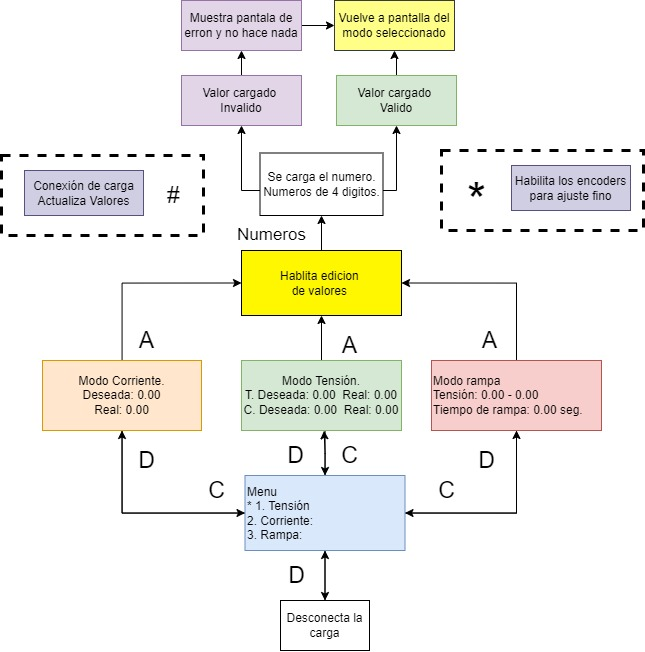
\includegraphics[scale=0.6]{./imagenes/MoverseSobreMenu.jpg}
    \caption{Diagrama de bloques del funcionamiento estándar.}
    \label{F:funcionamiento_normal}
\end{figure}

\section{Uso de teclado} 
El teclado es una interfaz fundamental en el proceso de interacción del usuario con la fuente de alimentación, permitiendo la configuración de parámetros y el control de diferentes modos de operación. Cada tecla tiene asignada una función específica para facilitar la navegación y la manipulación de la configuración. A continuación, se presenta un resumen de la función que realiza cada tecla:
\begin{itemize}
    \item A: Editar valores.
    \item B: Moverse sobre el menú.
    \item C: Confirmar.
    \item D: Volver atrás.
    \item *: Alternar entre teclado y \textit{encoder} para la configuración de la referencia.
    \item \#: Poner en marcha el modo.
    \item Número: Valores numéricos.
\end{itemize}
Estas funciones se ven representadas en la Figura \ref{F:funcionamiento_normal} donde se muestra como con la pulsación de una tecla se genera la transición entre una pantalla a otra.

\section{Pantallas Disponibles} 
En el display se encuentran disponibles seis pantallas distintas, cada una con un propósito específico para la interacción del usuario con la fuente. A continuación, se detalla el contenido y la función de cada una. \par 
Esta estructura proporciona al usuario una interfaz intuitiva y clara para interactuar con la fuente, facilitando la configuración y el monitoreo de los parámetros de salida.\par 
\begin{enumerate}
    \item \textbf{Pantalla Principal - Menú Principal}: Esta pantalla representa el menú principal desde el cual se puede navegar para configurar la fuente. Mediante un puntero, el usuario puede seleccionar el modo de operación deseado.
    \item \textbf{Pantalla de Modo Tensión}: Al seleccionar este modo, la pantalla mostrará los valores configurados de tensión y corriente. Además, proporcionará una visualización en tiempo real de las magnitudes de registradas a tiempo real que se actualiza cada un segundo.
    \item \textbf{Pantalla de Modo Corriente}: Similar al modo de tensión, esta pantalla muestra los valores configurados para la corriente. No incluye un campo para la tensión deseada, ya que se activa exclusivamente el modo de corriente.
    \item \textbf{Pantalla de Modo Rampa}: Aquí se visualizan los valores de tiempo y tensión configurados, junto con los valores registrados en tiempo real y el tiempo transcurrido desde el inicio del modo de rampa.
    \item \textbf{Pantalla de Carga Inválida}: Esta pantalla muestra un mensaje de error cuando los parámetros cargados no son válidos dentro de los límites constructivos de la fuente.
    \item \textbf{Pantalla de Carga de Valores}: En esta pantalla se muestran los valores deseados de los parámetros. Se pueden cargar uno a la vez utilizando el teclado alfanumérico.
    \item \textbf{Pantalla de Error}: Ocurrido algún fenómeno que dispare el valor de corriente a uno superior al configurado en la protección, indicará al usuario de este acontecimiento además de bloquear el funcionamiento normal.
\end{enumerate}

\section{Rangos límite y zonas de operación}
A su vez se han establecido los valores límites mínimos y máximos para garantizar la operación adecuada de la fuente de alimentación y la implementación efectiva del algoritmo de control. Estos valores son los siguientes:

\begin{table}[h!]
\centering
\begin{tabular}{|c|c|c|c|c|c|}
\hline
    \textbf{Modo}   & \multicolumn{2}{c|}{\textbf{Tensión}} & \multicolumn{1}{c|}{\textbf{Corriente}} & \multicolumn{2}{c|}{\textbf{Rampa}} \\ \hline
       & \textbf{Tensión}  & \textbf{Corriente} & \textbf{Corriente} & \textbf{Tensión} & \textbf{Tiempo} \\ \hline
\textbf{Máximo} &30V            &3A             &3A                &30V             &2s               \\ \hline
\textbf{Mínimo} &3V             &200mA          &200mA             &3V              &2s               \\ \hline
\end{tabular}
\caption{Rangos máximos y mínimos de operación para los diferentes modos.}
\end{table}











